\documentclass[10pt, a4paper]{article}

% On écrit en français
\usepackage[utf8]{inputenc}
\usepackage[frenchb]{babel}
\usepackage[T1]{fontenc}

% Packages nécessaires
\usepackage{graphicx}
\usepackage{hyperref}

% Numérotation de page custom
\usepackage{fancyhdr}
\usepackage{lastpage}
\pagestyle{fancy}
\fancyhf{}
\rfoot{Page \thepage \hspace{1pt} sur \pageref{LastPage}}

% Police Helvetica <3
\usepackage{helvet}
\renewcommand*{\familydefault}{\sfdefault}

% Enlever les alinéas
\setlength{\parindent}{0pt}

% Marges plus larges pour faire moins LaTeX
\usepackage[left=3cm, right=3cm]{geometry}

% Sous titre de document
\usepackage{titling}
\newcommand{\subtitle}[1]{%
  \posttitle{%
    \par\end{center}
    \begin{center}\large#1\end{center}
    \vskip0.5em}%
}

% En tête complet de document
\newcommand{\Document}[1]{%
    \title{#1}
    \subtitle{Dématérialisation d'un processus de paiement}
    \author{
        COMETS Jean-Marie \\
        DELMARRE Adrian \\
        REYNOLDS Nicolas \\
        TURPIN Pierre
    }
    \date{\today}

    \maketitle \newpage

    \tableofcontents \newpage
}


\begin{document}

\Document{Architecture technique}

\section{Présentation générale}

La figure \ref{fig:network} détaille l'architecture technique choisie.
Cependant, certains points doivent être justifiés ou davantage expliqués.

\begin{figure}[htpb]
    \centering
    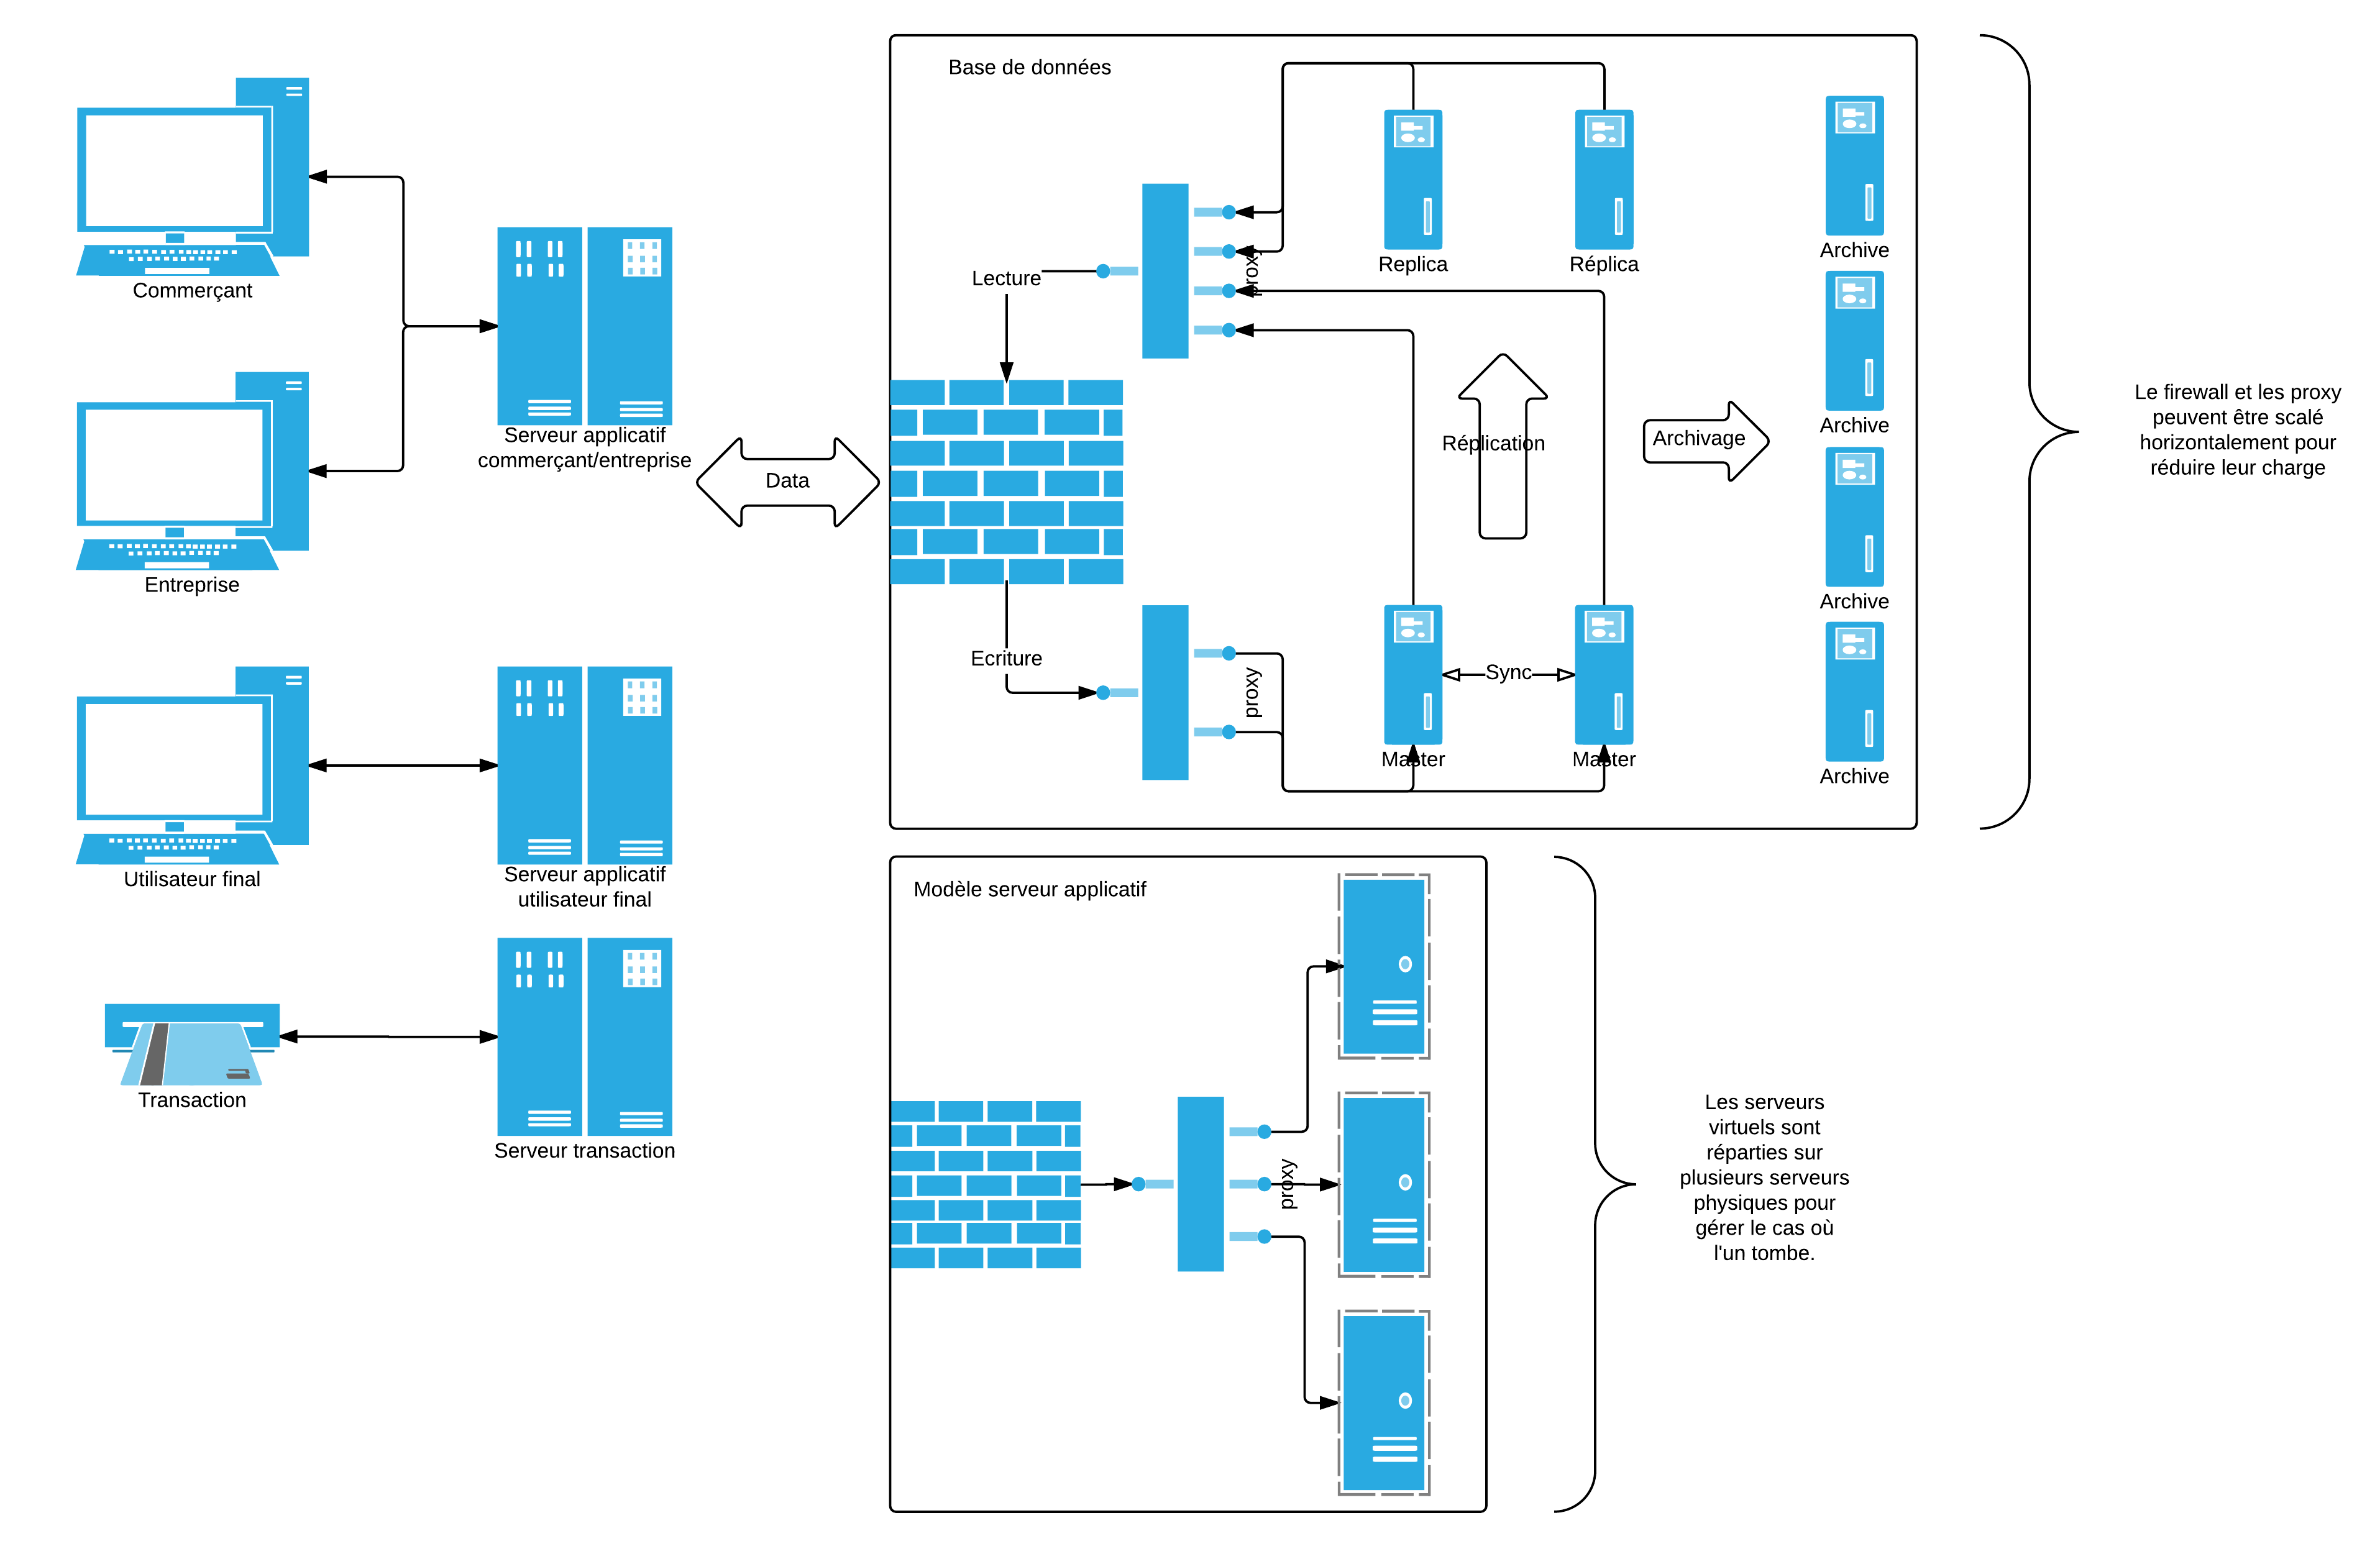
\includegraphics[width=\textwidth]{network}
    \caption{Schéma général de l'architecture technique choisie}
    \label{fig:network}
\end{figure}

\paragraph{Serveurs applicatifs}

L'accés aux serveurs applicatifs est gouverné par une couche \textbf{firewall}
et une couche \textbf{proxy}. La couche firewall est nécessaire pour gérer le
trafic indésirable (se référer à la section
\ref{subsec:gestion-trafic-indesirable} pour plus de détails). La couche proxy
permet de gérer le passage à l'échelle des serveurs applicatifs. \\

Le principe général du passage à l'échelle des serveurs applicatifs est basé
sur la duplication et synchronisation de plusieurs instances des serveurs
applicatifs, avec balance de charge sur ces dernières, régie par le proxy (se
référer à la section {\huge \textbf{TODO} } pour plus de détails).

\paragraph{Base de données}

L'accés au sous-système de base de données est régi par un deuxième firewall,
spécifiquement conçu pour le SGBD choisi. L'idée est de bloquer l'accés au
sous-système de base de données au monde extérieur, autorisant uniquement
l'accés au proxy servant à répartir les accés aux différentes base de données
"maîtres". \\

\section{Choix de la solution cloud}
\label{sec:choix-solution-cloud}
\section{Passage à l'échelle (scaling)}
\label{sec:scaling}

\section{Sécurité}
\label{sec:securite}

\subsection{Sécurité d'infrastructure}
\label{subsec:securite-infrastructure}

En choisissant une solution cloud, la disponibilité de l'infrastructure est
garantie par le prestataire cloud, en l'occurence \textbf{Amazon AWS}. Le
système peut donc être considéré relativement sécurisé vis-à-vis des attaques
par déni de service (DoS simple), ou autre attaque d'infrastructure. \\

De plus, la disponibilité du système est dépendante de la disponibilité d'AWS,
en l'occurence celle-ci peut être assurée selon le prix de la prestation. Le
taux de panne de 0\% ne peut malheureusement pas l'être, du fait du nombre de
facteurs externes entrant en jeu. Cependant, un taux de 99\%, voire jusqu'à
99.95\% peut l'être par AWS (source: \url{http://aws.amazon.com/ec2/sla/}). \\

En passant par une solution cloud, le système est aussi protégé des attaques
physiques (coupure générale, attaque électromagnétique, etc...), mais encore
dépendant de l'infrastructure d'AWS.

\begin{figure}[h]
    \centering
    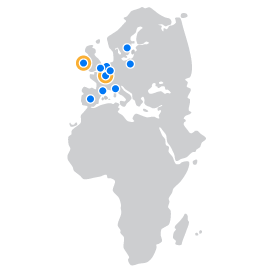
\includegraphics[width=0.7\textwidth]{aws-europe}
    \caption{Emplacements géographiques possibles des instances EC2}
    \label{fig:aws-europe}
\end{figure}

\subsection{Gestion du trafic indésirable}
\label{subsec:gestion-trafic-indesirable}

Le trafic indésirable correspond au trafic qui n'est pas directement lié à
l'utilisation normale du système. Il peut être utilisé comme attaque visant à
réduire exploiter des failles d'autres services présents sur la VM, ou tout
simplement visant à réduire la disponibilité du système en multipliant les
accés (DoS). \\

EC2 met à disposition un firewall pour ses instances, ce qui permet de régler
son accés. Cependant, les VM étant installées à l'intérieur d'une instance,
elles doivent toutes être configurées séparément pour accepter uniquement le
trafic qui les concerne.

\paragraph{Fermeture maximale}

Un document relatant des conseils de sécurisation d'instance EC2, produit par
ce même service, est disponible à l'adresse suivante :
\url{http://aws.amazon.com/articles/1233/} (en date du \today). L'idée est
simplement de n'autoriser que le trafic qui est attendu, et par défaut de
bloquer toute connexion entrante ne correspondant pas à une règle spécifiée.

\paragraph{Surcouche base de données}

Pour garantir la sécurité des données, une surcouche firewall est ajoutée au
bloc "base de données. Dans le cas où un des systèmes applicatifs serait
compromis, ce pare-feu supplémentaire limitera l'ampleur des dégâts (pas
d'accés aux archives par exemple).

\end{document}
